% Options here are passed to the article class.
% Most common options: 10pt, 11pt, 12pt
\documentclass[10pt]{datasheet}

% Input encoding and typographical rules for English language
\usepackage[utf8]{inputenc}
\usepackage[english]{babel}
\usepackage[english]{isodate}

% tikz is used to draw images in this example, but you can
% also use \includegraphics{}.
\usepackage{graphicx}

% These define global texts that are used in headers and titles.
\title{LC07: Decimal Delay Generator}
\author{Andrews54757}
\tags{logic-and-computation, decimal, variable-delay}
\date{21 December 2023}
\revision{Revision 1}
\begin{document}
\maketitle

\section{Features}

\begin{itemize}
\item{10gt to 19gt variable delay}
\item{SS5-14 input}
\item{Not random activation timings safe}
\end{itemize}

\section{Applications}

\begin{itemize}
\item{Slot iterator device for dynamic bulk code mappings storage.}
\end{itemize}

\section{General Description}

The LC07 Decimal Delay Generator takes a decimal input and outputs a pulse after a delay of 10 to 19 game ticks. The delay is equal to the input signal strength plus 5. The device can be used to generate precise extraction trigger signal for a 1 slot/gt iterator device.

\vfill\break

\begin{figure}[h]
    \centering
    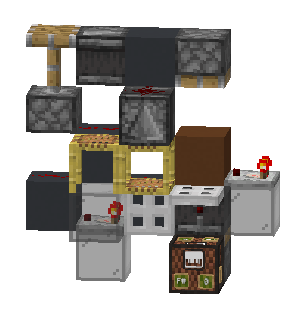
\includegraphics[width=0.48\textwidth]{decimaldelay.png}
    \caption{\centering Decimal Delay Generator}
\end{figure}

% For wide tables, a single column layout is better. It can be switched
% page-by-page.
\onecolumn

\section{Device Specifications}

\begin{table}[h]
    \caption{Inputs}
    \begin{tabularx}{\textwidth}{l | c | X}
        \thickhline
        \textbf{Name} & \textbf{Range} & \textbf{Description} \\
        \hline
        Decimal input & 5-14 & Determines length of delay. Delay is signal strength $+ 5gt$ \\
        \hline
        Input trigger & Pulse & Starts the delay generator \\
        \thickhline
\end{tabularx}
\end{table}

\begin{table}[h]
    \caption{Outputs}
    \begin{tabularx}{\textwidth}{l | c | X}
        \thickhline
        \textbf{Name} & \textbf{Range} & \textbf{Description} \\
        \hline
        Delayed trigger & Pulse & Delayed output pulse \\
        \thickhline
\end{tabularx}
\end{table}

\begin{table}[h]
    \caption{Device Specifications}
    \begin{tabularx}{\textwidth}{l | c c c | c | X}
        \thickhline
        \textbf{Parameter} & \textbf{Min.} & \textbf{Typ.} & \textbf{Max.} &
        \textbf{Unit} & \textbf{Conditions} \\
        \hline
        Throughput  & 22 & - & - & gt & Normal Usage \\
        \hline
        Delay    & 10 & - & 19 & gt & From input to dropper activation. \\
        \hline
        MC Version & 1.16 & 1.19.3 & - & MCV & Latest version at time of writing: 1.20.4\\
        \hline
        Dimensions & & 4 x 5 x 2 & & Blocks & \\
        \thickhline
\end{tabularx}
\end{table}
\newpage
\section{Testing Data}
\begin{table}[h]
\caption{Executed Tests}
\begin{tabularx}{\textwidth}{l | X}
    \thickhline
    \textbf{Test} & \textbf{Result} \\
    \hline
    Delay test & Device was able to produce all delays ranging from 10 to 19 gt as determined by the input signal strength.\\
    \hline
    Failed random timings test & Device was unable to survive random activation timings. A slider became stuck in the wrong state.\\
    \thickhline
\end{tabularx}
\end{table}

\section{Download Information}
\begin{table}[h]
    \caption{Download Information}
    \begin{tabularx}{\textwidth}{l | l | l | X}
        \thickhline
        \textbf{Identifier} & \textbf{MC} & \textbf{File} & \textbf{Description} \\
        \hline
        LC07 & 1.19.3 & \href{https://github.com/Soontech-Annals/Archive/blob/b56572c0d2b4f182d9e9d41449d8cb2963b923ae/Archive/logic-and-computation/LC07\%20Decimal\%20Delay\%20Generator/LC07\_Decimal\_Delay\_Generator.litematic?raw=1}{LC07\_Decimal\_Delay\_Generator.litematic} & Schematic of device. Test input regions included. \\
        \hline
        \thickhline
    \end{tabularx}
\end{table}

\end{document}

